% Main source of the project report.
% Build:  python <plugin>/skills/write-report/scripts/build_report.py report
%    or:  latexmk -pdf -interaction=nonstopmode -halt-on-error main.tex
\documentclass[12pt,a4paper]{report}

% --- Fonts, language, layout ----------------------------------------------
\usepackage[T1]{fontenc}
\usepackage[utf8]{inputenc}
\usepackage{lmodern}
\usepackage[english]{babel}
\usepackage{csquotes}
\usepackage{microtype}
\usepackage[margin=2cm,headheight=16pt,headsep=18pt]{geometry}
\usepackage{setspace}
\setstretch{1.4}

% --- Figures, tables, maths -------------------------------------------------
\usepackage{graphicx}
\graphicspath{{figures/}}
\usepackage{amsmath,amssymb}
\usepackage{booktabs,tabularx,longtable,array}
\usepackage[font=small,labelfont=bf]{caption}
\usepackage{float}
\usepackage{xcolor}
\usepackage{tikz}
\usetikzlibrary{arrows.meta,shapes.geometric}

% --- Headers and footers ----------------------------------------------------
\usepackage{fancyhdr}
\pagestyle{fancy}
\fancyhf{}
\fancyhead[R]{\small\nouppercase{\textit{\leftmark}}}
\fancyfoot[C]{\thepage}
\renewcommand{\headrulewidth}{0.4pt}
\renewcommand{\chaptermark}[1]{\markboth{#1}{}}
\fancypagestyle{plain}{%
  \fancyhf{}\fancyfoot[C]{\thepage}%
  \renewcommand{\headrulewidth}{0pt}%
}

% --- Contents and bibliography ----------------------------------------------
\usepackage[nottoc,notbib]{tocbibind}   % lists of figures/tables in the TOC
\usepackage[backend=biber,style=numeric,sorting=none]{biblatex}
\addbibresource{references.bib}

\usepackage{hyperref}                   % keep hyperref last
\hypersetup{colorlinks=true,linkcolor=black,citecolor=magenta,urlcolor=magenta,
            pdftitle={Project Report}}  % TODO: set the real title

% --- Report macros ----------------------------------------------------------
% \toverify{...}: visible red marker for a statement that still needs evidence.
\newcommand{\toverify}[1]{\textcolor{red}{\textbf{[TO VERIFY: #1]}}}

% \crispdm{ID}: marks the section that addresses CRISP-DM generic task ID
% (BU.1 ... DE.4). Place it right under the section heading.
% \crispdm[na]{ID}: the task does not apply; the section explains why.
% Both print nothing. They feed the traceability table (\crisploc) and the
% crisp_dm_check.py coverage checker. Only the first marker of an ID gets the label.
\newcommand{\crispdm}[2][]{%
  \ifcsname crispdm@seen@#2\endcsname\else
    \expandafter\gdef\csname crispdm@seen@#2\endcsname{}\label{crisp:#2}%
  \fi}
% \crisploc{ID}: "§ 3.4.1, p. 23", used in the traceability table.
\newcommand{\crisploc}[1]{\S\,\ref{crisp:#1}, p.~\pageref{crisp:#1}}

\begin{document}

% --- Front matter (Roman page numbers) --------------------------------------
\pagenumbering{roman}
% Include these only when the institution requires them or the author supplies
% the wording. Never invent names, supervisors or host organizations.
% % Cover page: include only if the institution requires one, and prefer its
% official template when it provides one. Every field comes from the author;
% never guess names, institutions or dates.
\begin{titlepage}
  \centering
  {\large \toverify{University or school}\par}
  {\normalsize \toverify{Department or programme}\par}
  \vspace{2.5cm}
  {\large \toverify{Report type, e.g. End-of-Studies Project Report}\par}
  \vspace{1cm}
  \rule{\textwidth}{0.6pt}\par\vspace{0.4cm}
  {\LARGE\bfseries \toverify{Report title}\par}
  \vspace{0.4cm}\rule{\textwidth}{0.6pt}\par
  \vspace{2cm}
  {\large Presented by\par \toverify{Author}\par}
  \vfill
  \begin{tabular}{@{}ll@{}}
    Supervisor: & \toverify{Name, affiliation} \\
  \end{tabular}\par
  \vspace{1cm}
  {\normalsize Academic year \toverify{YYYY--YYYY}\par}
\end{titlepage}

% \input{chapters/dedication}        % create this file first if wanted
% \chapter*{Acknowledgements}
\phantomsection\addcontentsline{toc}{chapter}{Acknowledgements}
\markboth{Acknowledgements}{}

% Only with names and wording supplied by the author.

\chapter*{List of Abbreviations}
\phantomsection\addcontentsline{toc}{chapter}{List of Abbreviations}
\markboth{List of Abbreviations}{}

% Alphabetical. Only abbreviations that actually appear in the report.
% Switch to longtable if the list runs past one page.
\noindent
\begin{tabular}{@{}p{0.22\textwidth}p{0.72\textwidth}@{}}
\textbf{Abbreviation} & \textbf{Meaning} \\
\midrule
CRISP-DM & Cross-Industry Standard Process for Data Mining \\
\end{tabular}

\chapter*{Abstract}
\phantomsection\addcontentsline{toc}{chapter}{Abstract}
\markboth{Abstract}{}

% Write this LAST, once the results are final.
% 150-250 words in one or two paragraphs: problem, goal, method (CRISP-DM),
% what was implemented, evaluation evidence with the key numbers, conclusion,
% main limitation. Every number must match Chapter 4 exactly.

\bigskip
\noindent\textbf{Keywords:} % 5-10 precise keywords separated by semicolons.

\tableofcontents
\listoffigures
\listoftables

% --- Main matter (Arabic page numbers restart at 1) -------------------------
\clearpage
\pagenumbering{arabic}
\chapter*{General Introduction}
\phantomsection\addcontentsline{toc}{chapter}{General Introduction}
\markboth{General Introduction}{}
% DE.3 (Produce final report): this report is the final CRISP-DM deliverable.
% Say so in the paragraph that presents the organization of the report.
\crispdm{DE.3}

% 1. The broad field, in two or three sentences about THIS project's domain.
% 2. The concrete problem and why current practice is insufficient.
% 3. What the project proposes and builds.
% 4. The methodology in one sentence: CRISP-DM, cited.
% 5. Organization of the report: one sentence per chapter, ending with the
%    General Conclusion. Mention that the report itself is the final
%    deliverable of the CRISP-DM deployment phase.

\chapter{Project Overview and Context}
\label{chap:context}
% This chapter covers the CRISP-DM Business Understanding phase (BU.1-BU.4).
% Most of it comes from the author, not the code: ask, then mark gaps with \toverify.

\section{Introduction}
% What this chapter answers: why the project exists. Two or three sentences.

\section{Project and Organization Context}
% Only if there is a host organization or client. Otherwise delete this section.
% Never invent a company, team or supervisor.

\section{General Context and Motivation}
% The domain and the real-world situation that motivates the project.

\section{Problem Statement}
% The precise problem, who experiences it, and why existing practice falls short.

\section{Business Objectives and Success Criteria}
\crispdm{BU.1}
% BU.1 Determine business objectives.
% Background, objectives in BUSINESS terms (not "train a model"), and measurable
% business success criteria. Each criterion must be evaluated again in
% Chapter 4 (Section~\ref{sec:business-evaluation}).

\section{Situation Assessment}
\crispdm{BU.2}
% BU.2 Assess situation.
% Resources (people, data, hardware, software), requirements, assumptions and
% constraints (deadline, privacy, compute, data access), risks and
% contingencies (a short table works well), key terminology, and costs and
% benefits (qualitative if no figures exist; never invent budgets).

\section{Data Mining Goals and Success Criteria}
\crispdm{BU.3}
% BU.3 Determine data mining goals.
% Translate the business objectives into a technical task (classification,
% detection, regression, forecasting, ...), with inputs, outputs and technical
% success criteria (metric + threshold + data split). If no threshold was fixed
% before the experiments, say so honestly.

\section{Project Plan}
\crispdm{BU.4}
% BU.4 Produce project plan.
% Phases and milestones; a Gantt chart only from real dates (git history can
% help), otherwise label it "proposed". Initial assessment of tools and
% techniques, with a pointer to Chapter~\ref{chap:sota} for the justification.

\section{Conclusion}
% Summarize the context and objectives; transition to the state of the art.

\chapter{State of the Art}
\label{chap:sota}
% What others have done, and why this project's approach was chosen.
% Every external claim needs a verified citation in references.bib.

\section{Introduction}

\section{Literature Review}
% Research papers on the problem and on the candidate techniques.

\section{Existing Solutions and Tools}
% Products, open-source repositories, frameworks and libraries.

\section{Comparative Analysis}
% A comparison table with explicitly defined criteria, citing the source of
% every value. No invented scores and no universal "best" claims.

\section{Justification of the Proposed Approach}
% Why these techniques and tools fit this project's constraints (Section on the
% situation assessment in Chapter~\ref{chap:context}). This supports BU.4
% (initial assessment of tools and techniques) and MO.1 (modeling technique).

\section{Conclusion}
% Transition to the methodology.

\chapter{Methodology and System Design}
\label{chap:methodology}
% How the project works and how it was built: the most reproducible chapter.
% Covers CRISP-DM Data Understanding, Data Preparation, Modeling (MO.1, MO.3)
% and Deployment planning (DE.1, DE.2). MO.2 and MO.4 are in Chapter 4.

\section{Introduction}

\section{Development Methodology: CRISP-DM}
\label{sec:crispdm}
The project follows the Cross-Industry Standard Process for Data Mining
(CRISP-DM)~\cite{chapman2000crisp,wirth2000crisp}, which organizes a data
project into six phases (business understanding, data understanding, data
preparation, modeling, evaluation and deployment), each broken down into
generic tasks with defined outputs. The phases are not executed strictly in
sequence: the process explicitly allows returning to an earlier phase when a
later one reveals a problem, as shown in Figure~\ref{fig:crispdm-cycle}.

% Then, about THIS project:
% - why CRISP-DM rather than an alternative such as the KDD process
%   \cite{fayyad1996kdd} (cite only verified sources);
% - how it was adapted (e.g. which tasks were light or not applicable);
% - the iterations that ACTUALLY happened between phases, with evidence
%   (experiment logs, git history). Do not invent loops.
% - a pointer to Table~\ref{tab:crispdm-traceability}, which maps every
%   generic task to the section of this report that addresses it.

\begin{figure}[htbp]
  \centering
  % CRISP-DM process model, redrawn after Chapman et al. (2000).
% Needs: \usepackage{tikz} and \usetikzlibrary{arrows.meta,shapes.geometric}.
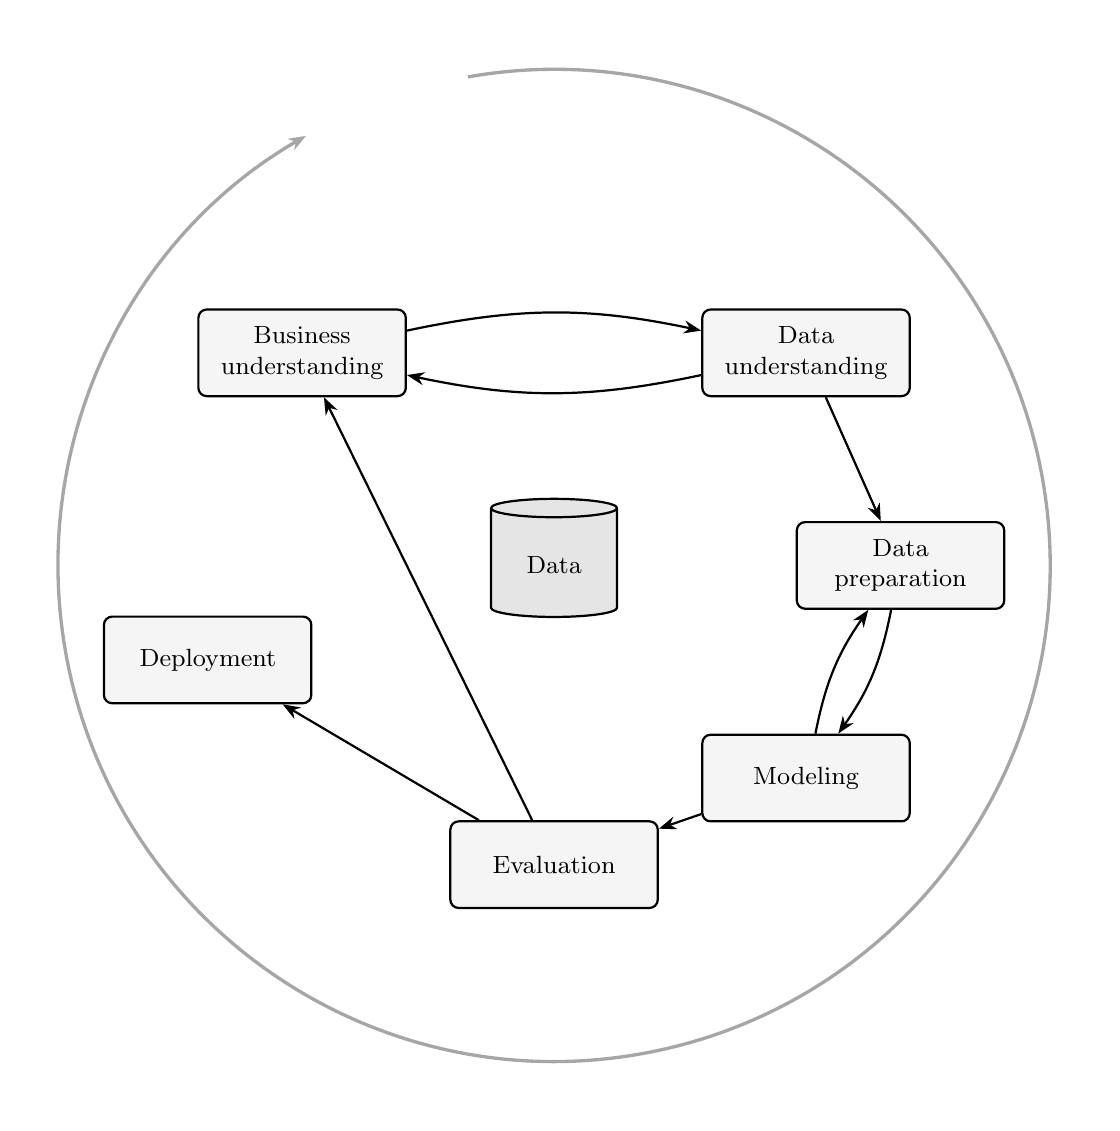
\begin{tikzpicture}[
    font=\small,
    phase/.style={draw, thick, rounded corners=3pt, fill=gray!8, align=center,
                  text width=2.4cm, minimum height=1.1cm},
    flow/.style={-{Stealth[length=2.2mm]}, thick},
  ]
  \node[draw, thick, cylinder, shape border rotate=90, aspect=0.25,
        fill=gray!20, minimum width=1.6cm, minimum height=1.5cm] (data) at (0,0) {Data};

  \node[phase] (bu) at (-3.2, 2.7) {Business\\understanding};
  \node[phase] (du) at ( 3.2, 2.7) {Data\\understanding};
  \node[phase] (dp) at ( 4.4, 0.0) {Data\\preparation};
  \node[phase] (mo) at ( 3.2,-2.7) {Modeling};
  \node[phase] (ev) at ( 0.0,-3.8) {Evaluation};
  \node[phase] (de) at (-4.4,-1.2) {Deployment};

  % Transitions of the reference model; paired arrows mean frequent back-and-forth.
  \draw[flow] (bu) to[bend left=12] (du);
  \draw[flow] (du) to[bend left=12] (bu);
  \draw[flow] (du) -- (dp);
  \draw[flow] (dp) to[bend left=12] (mo);
  \draw[flow] (mo) to[bend left=12] (dp);
  \draw[flow] (mo) -- (ev);
  \draw[flow] (ev) -- (bu);
  \draw[flow] (ev) -- (de);

  % Outer cycle: data projects iterate.
  \draw[flow, gray!70, line width=1.2pt]
    (100:6.3) arc[start angle=100, end angle=-240, radius=6.3];
\end{tikzpicture}

  \caption[The CRISP-DM process model]{The six phases of the CRISP-DM process
    model and the main transitions between them; the outer arrow denotes the
    cyclic nature of data projects (redrawn after~\cite{chapman2000crisp}).}
  \label{fig:crispdm-cycle}
\end{figure}

% Traceability of the 24 CRISP-DM generic tasks to this report.
% The last column fills itself from the \crispdm{ID} markers: do not type
% section numbers by hand. DE.3 and DE.4 live in unnumbered chapters, so they
% link by name instead of by section number.
\begingroup
\setstretch{1.05}\small
\begin{longtable}{@{}p{0.23\textwidth}p{0.07\textwidth}p{0.38\textwidth}p{0.22\textwidth}@{}}
\caption[Traceability of the CRISP-DM generic tasks to this report]{Traceability
  of the CRISP-DM generic tasks~\cite{chapman2000crisp} to the sections of this
  report.}
\label{tab:crispdm-traceability}\\
\toprule
\textbf{Phase} & \textbf{ID} & \textbf{Generic task} & \textbf{Addressed in} \\
\midrule
\endfirsthead
\multicolumn{4}{@{}l}{\itshape Table~\ref{tab:crispdm-traceability} (continued)} \\
\toprule
\textbf{Phase} & \textbf{ID} & \textbf{Generic task} & \textbf{Addressed in} \\
\midrule
\endhead
\bottomrule
\endlastfoot
Business understanding & BU.1 & Determine business objectives & \crisploc{BU.1} \\
                       & BU.2 & Assess situation & \crisploc{BU.2} \\
                       & BU.3 & Determine data mining goals & \crisploc{BU.3} \\
                       & BU.4 & Produce project plan & \crisploc{BU.4} \\
\midrule
Data understanding     & DU.1 & Collect initial data & \crisploc{DU.1} \\
                       & DU.2 & Describe data & \crisploc{DU.2} \\
                       & DU.3 & Explore data & \crisploc{DU.3} \\
                       & DU.4 & Verify data quality & \crisploc{DU.4} \\
\midrule
Data preparation       & DP.1 & Select data & \crisploc{DP.1} \\
                       & DP.2 & Clean data & \crisploc{DP.2} \\
                       & DP.3 & Construct data & \crisploc{DP.3} \\
                       & DP.4 & Integrate data & \crisploc{DP.4} \\
                       & DP.5 & Format data & \crisploc{DP.5} \\
\midrule
Modeling               & MO.1 & Select modeling technique & \crisploc{MO.1} \\
                       & MO.2 & Generate test design & \crisploc{MO.2} \\
                       & MO.3 & Build model & \crisploc{MO.3} \\
                       & MO.4 & Assess model & \crisploc{MO.4} \\
\midrule
Evaluation             & EV.1 & Evaluate results & \crisploc{EV.1} \\
                       & EV.2 & Review process & \crisploc{EV.2} \\
                       & EV.3 & Determine next steps & \crisploc{EV.3} \\
\midrule
Deployment             & DE.1 & Plan deployment & \crisploc{DE.1} \\
                       & DE.2 & Plan monitoring and maintenance & \crisploc{DE.2} \\
                       & DE.3 & Produce final report &
  \hyperref[crisp:DE.3]{General Introduction}, p.~\pageref{crisp:DE.3} \\
                       & DE.4 & Review project &
  \hyperref[crisp:DE.4]{General Conclusion}, p.~\pageref{crisp:DE.4} \\
\end{longtable}
\endgroup


\section{System Architecture and Workflow}
% A high-level box-and-arrow diagram of the real pipeline (data sources ->
% preparation -> model -> outputs/integration) BEFORE the details below.

\section{Data Understanding}
% CRISP-DM phase 2. Numbers must be computed from the actual data.

\subsection{Initial Data Collection}
\crispdm{DU.1}
% DU.1 Sources, acquisition method and date, licence or permission, provenance,
% problems met during collection.

\subsection{Data Description}
\crispdm{DU.2}
% DU.2 Format, volume, schema/fields with types and units, classes and counts,
% time span. A table is usually clearest.

\subsection{Data Exploration}
\crispdm{DU.3}
% DU.3 Distributions, class balance, correlations, representative (anonymized)
% samples, and the findings that shaped later decisions.

\subsection{Data Quality Verification}
\crispdm{DU.4}
% DU.4 Missing values, label noise, duplicates, outliers, inconsistencies and
% bias, quantified. Every issue listed here is handled in Data Cleaning.

\section{Data Preparation}
% CRISP-DM phase 3.

\subsection{Data Selection}
\crispdm{DP.1}
% DP.1 What was kept or excluded (records, attributes, time ranges) and why.

\subsection{Data Cleaning}
\crispdm{DP.2}
% DP.2 For each quality issue from the previous phase: action taken and its
% effect (counts before/after), or why it was left alone.

\subsection{Data Construction and Feature Engineering}
\crispdm{DP.3}
% DP.3 Derived attributes (with formulas), augmentation or generated records
% (technique, parameters), and the reason for each.

\subsection{Data Integration}
\crispdm{DP.4}
% DP.4 How sources were merged (keys, conflicts). With a single source, change
% the marker to \crispdm[na]{DP.4} and explain in one or two sentences.

\subsection{Data Formatting}
\crispdm{DP.5}
% DP.5 Format conversions required by the modeling tools (label format,
% resizing, normalization, encoding, file layout) and a short description of
% the final dataset handed to modeling.

\section{Modeling}
% CRISP-DM phase 4. The test design (MO.2) and the model assessment (MO.4) are
% reported in Chapter 4; point to them here.

\subsection{Selection of Modeling Techniques}
\crispdm{MO.1}
% MO.1 Candidate techniques, the choice and its reasons (link to
% Chapter~\ref{chap:sota}), and the assumptions the technique makes.

\subsection{Model Building}
\crispdm{MO.3}
% MO.3 Architecture, hyperparameter table, training procedure (epochs,
% optimizer, schedule, seeds), hardware, training time, and training curves
% drawn from the real logs.

\section{Deployment and Integration}
% CRISP-DM phase 6 (planning). Keep "implemented", "prototype" and "planned"
% distinct. Never claim production use that was not demonstrated.

\subsection{Deployment Plan}
\crispdm{DE.1}
% DE.1 How the model reaches its users (API, application, edge device, batch
% job): what is implemented versus proposed; an integration diagram if useful.

\subsection{Monitoring and Maintenance Plan}
\crispdm{DE.2}
% DE.2 What would be monitored (input drift, prediction quality, latency),
% retraining triggers and ownership. Usually a proposal: label it as such.

\section{Conclusion}
% Summarize the methodology; transition to the results.

\chapter{Results and Discussion}
\label{chap:results}
% What was demonstrated and how well it worked. Only real measurements.
% Covers CRISP-DM MO.2, MO.4 and the Evaluation phase (EV.1-EV.3).

\section{Introduction}

\section{Experimental Setup and Test Design}
\crispdm{MO.2}
% MO.2 Generate test design, decided BEFORE assessing models.
% Exact environment (hardware, software versions, dates), data split
% (proportions, stratification, temporal/group split, leakage prevention),
% validation protocol, baseline, and how the test set was kept untouched.
% Split sizes must add up with the data description in Chapter 3.

\section{Evaluation Metrics}
% Each metric as a numbered equation with every variable defined, plus a
% plain-language explanation of what it rewards or penalizes.

\section{Model Assessment}
\crispdm{MO.4}
% MO.4 Assess model: results per split (validation vs held-out test), variants
% compared, tuning iterations, against the technical criteria of Chapter 1.
% Plots and tables generated from the real logs only.

\section{Functional Demonstration}
% Qualitative evidence: real screenshots, example predictions, representative
% successes and failures (anonymized).

\section{Evaluation Against Business Success Criteria}
\label{sec:business-evaluation}
\crispdm{EV.1}
% EV.1 Evaluate results: for EACH business success criterion of Chapter 1, is
% it met, not met, or not measurable yet, and on what evidence? Which model is
% approved and why? This is a business judgement; do not just repeat the
% metrics above.

\section{Review of the Process}
\crispdm{EV.2}
% EV.2 Review process: error analysis, steps skipped or rushed, leakage checks,
% risks from the situation assessment that materialized, threats to validity,
% limitations.

\section{Discussion and Next Steps}
\crispdm{EV.3}
% EV.3 Determine next steps: the possible actions (deploy, iterate, collect more
% data, stop), the decision taken and its reasons. Must agree with the
% deployment plan and the General Conclusion.

\section{Conclusion}

\chapter*{General Conclusion and Future Work}
\phantomsection\addcontentsline{toc}{chapter}{General Conclusion and Future Work}
\markboth{General Conclusion and Future Work}{}

% Original objectives -> what was implemented -> what the evidence shows ->
% remaining limitations -> achievable next steps. No claims of deployment,
% production readiness or security guarantees that were not demonstrated.

\section*{Lessons Learned}
\crispdm{DE.4}
% DE.4 Review project (experience documentation): what worked, what did not,
% and what would be done differently, with specifics from this project.


\printbibliography[heading=bibintoc,title={Bibliography}]

% \appendix
% \input{chapters/appendix_a}

\end{document}
